\documentclass[a4paper,12pt]{article}

\usepackage[14pt]{extsizes}
\usepackage{cmap}					% поиск в PDF
\usepackage{mathtext} 				% русские буквы в формулах
\usepackage[T2A]{fontenc}			% кодировка
\usepackage[utf8]{inputenc}			% кодировка исходного текста
\usepackage[english,russian]{babel}	% локализация и переносы
\usepackage{graphicx}
\usepackage{geometry}
\usepackage{amsmath}
\usepackage{amssymb}
\usepackage[table]{xcolor}
\setlength\extrarowheight{2pt}


\geometry{verbose, a4paper, tmargin=2cm, bmargin=2cm, lmargin=3cm, rmargin=2cm}
\author{Vysotsky Maxim}
\title{Отчёт}
\date{2022}

\begin{document}
	\begin{titlepage}
		\begin{center}
			{Министерство науки и высшего образования Российской Федерации
				НОВОСИБИРСКИЙ НАЦИОНАЛЬНЫЙ ИССЛЕДОВАТЕЛЬСКИЙ
				ГОСУДАРСТВЕННЫЙ УНИВЕРСИТЕТ (НГУ)}
		\end{center}
		\begin{center}
			{Физический факультет}
		\end{center}
		\begin{center}
			{Кафедра общей физики}
		\end{center}
		
		
		\vspace{7cm}
		{
			\begin{center}
				{\bf Лабораторная работа №5.1}\\
				Измерение скорости звука в воздухе методом бегущей волны
			\end{center}
		}
		\vspace{2cm}
		\begin{flushright}
			{Руководитель:\\ Старший преподаватель\\
				Яцких А. А.\\
				Работу выполнил:\\
				Высоцкий М. Ю.\\
				\vspace{0.2cm}
				гр. 24301}
		\end{flushright}
		\vspace{3cm}
		\begin{center}
			Новосибирск, 2024
		\end{center}
	\end{titlepage}

\section{Теоретическое введение}
\textbf{Цель работы:} измерение зависимости амплитуды звуковой
волны от расстояния до источника, определение скорости звука в воз-
духе методом бегущей волны и скорости потока воздуха.

\textbf{Оборудование:} установка для измерения скорости звука методом
бегущей волны, генератор сигналов типа GFG 8255А, осциллограф типа TDS 1012, вентилятор.

\begin{figure}[ht!]
    \centering
    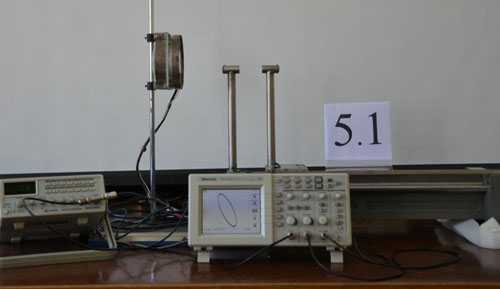
\includegraphics[scale=2.3]{ust.jpg}
    \caption{Фотография установки}
\end{figure}

\begin{figure}[ht!]
    \centering
    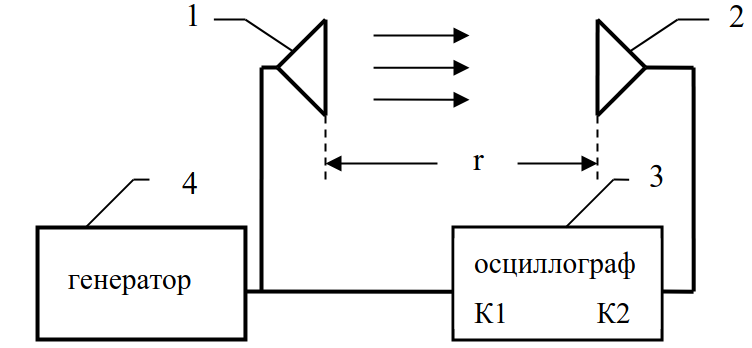
\includegraphics[scale=0.7]{scheme_1.jpg}
    \caption{Схема установки}
\end{figure}

\clearpage

\subsection{Задание 1. Измерение зависимости амплитуды волны от расстояния до источника.}

В данном задании нужно выставить частоту генератора около 40 кГц, затем снять зависимость амплитуды сигнала A от расстояния r между излучателем и приёмником. В пределах от 1 до 4 см шаг был 0,5 мм, а при дальней зоне от 5 до 30 см шаг был в 1 см. Для удобства, величина расстояний взята в миллиметрах. 

Также нужно отметить, что нуль расстояния между излучателем и приёмником на установке не соответствует нулю на линейке, он сдвинут на 1,5 мм, потому из всех значений r отнято именно это значение.

Данные будут приведены отдельным файлом, а графики покажем здесь.

\clearpage

\begin{figure}[ht!]
    \centering
    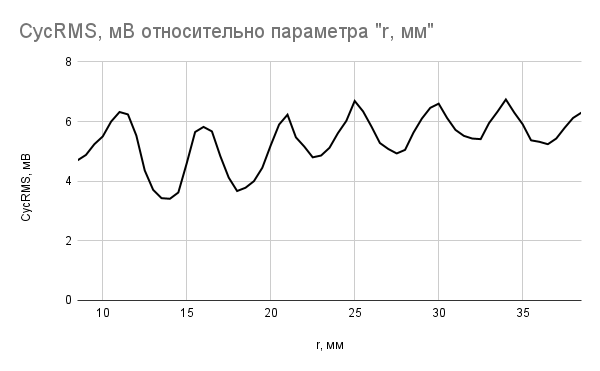
\includegraphics[scale=0.7]{ur_b.png}
    \caption{U(R), ближ.}
\end{figure}

\begin{figure}[ht!]
    \centering
    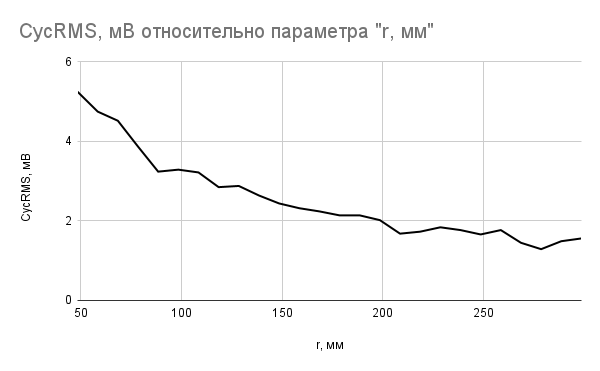
\includegraphics[scale=0.7]{ur_d.png}
    \caption{U(R), дал.}
\end{figure}

\clearpage

\begin{figure}[ht!]
    \centering
    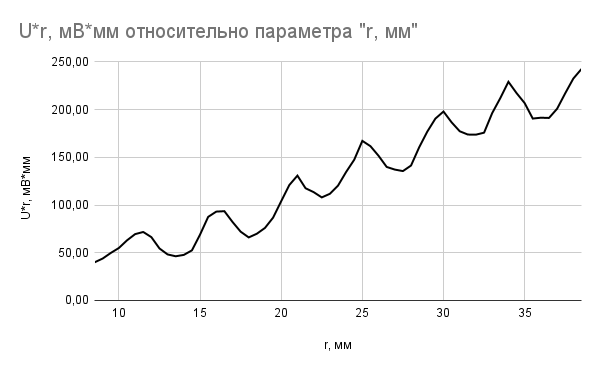
\includegraphics[scale=0.7]{urr_b.png}
    \caption{U*R(R), ближ.}
\end{figure}

\begin{figure}[ht!]
    \centering
    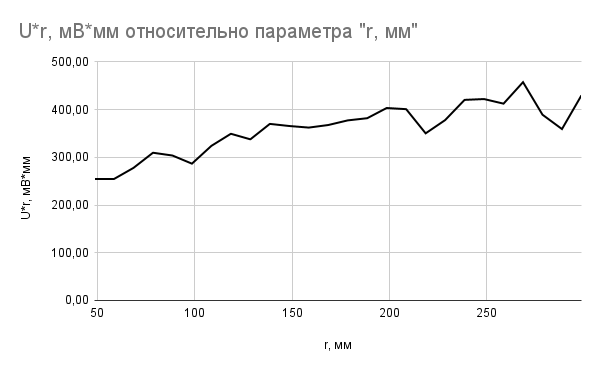
\includegraphics[scale=0.7]{urr_d.png}
    \caption{U*R(R), дал.}
\end{figure}
\clearpage

\subsection{Задание 2. Измерение скорости звука в воздухе.}

Мне лень писать задание. Нужно найти скорость звука, отодвигая приёмник, пока окружность не выродится 20 раз.

\begin{table}[!ht]
    \centering
    \begin{tabular}{|l|l|}
    \hline
        f, Гц & r, мм \\ \hline
        39,992 & 102,1 \\ \hline
        39,998 & 276,1 \\ \hline
    \end{tabular}
\end{table}

Длина волны $\lambda$ определяется: $$ \lambda = \frac{r_2-r_1}{20} = 8,7\hspace{0,1cm}мм$$

Скорость звука C определяется:
\begin{equation}
    C = \lambda f = 347,98 \pm 0,28\hspace{0,1cm}м/c 
\end{equation}
где пересчет погрешности: 
$$
    \Delta C = 2\Delta rf/20 + \Delta f(r_2-r_1)/20
$$

Температура в комнате была $26^{\circ}$ по Цельсию. После пересчета по формуле $$ C = \sqrt{T}*20,1$$ получается скорость звука порядка 347,85 м/c, что как раз попадает в наш интервал.

\clearpage

\subsection{Задание 3. Измерение скорости потока воздуха.}

Здесь надо было найти скорость потока воздуха.

\begin{table}[!ht]
    \centering
    \begin{tabular}{|l|l|l|l|l|l|l|}
    \hline
        фаза x & фаза y & у_0, В & у_м, В & х_0, В & х_м, В & r, mm \\ \hline
        0,80 & 1,12 & 9 & 10 & 7,2 & 10 & 64,6 \\ \hline
        0,85 & 1,09 & 8 & 9 & 7,2 & 9,6 & 81 \\ \hline
        0,43 & 0,52 & 3 & 6 & 4 & 9,6 & 108 \\ \hline
        1,02 & 0,99 & 5 & 6 & 9,2 & 10,8 & 128 \\ \hline
        0,57 & 0,85 & 3 & 4 & 5,2 & 9,6 & 153 \\ \hline
        0,64 & 1,02 & 3,4 & 4 & 6 & 10 & 188 \\ \hline
        0,85 & 1,12 & 3,6 & 4 & 7,2 & 9,6 & 204 \\ \hline
        1,12 & 0,93 & 3,2 & 4 & 3,6 & 4 & 251 \\ \hline
        0,59 & 0,70 & 4,5 & 7 & 5,36 & 9,6 & 99 \\ \hline
        0,83 & 1,29 & 4,8 & 5 & 7,32 & 9,92 & 134 \\ \hline
    \end{tabular}
\end{table}

Проведя все вычисления я получил скорость: $$
v = 3,96 \pm 0,75\hspace{0,1cm} м/c
$$

\end{document}